\part{\glqq Automatic Picture Transmition\grqq}
\section[Charakteristiken]{Einführung}
\begin{multicols}{2}

    Das Übertragungsverfahren \glqq Automatic Picture Transmition \grqq kurz APT ist ein analoges Bildübertragungsverfahren welches zuerst auf dem TIROS-8(Start 1963) Satelliten zur Anwendung kam und bis heute meist für Wetterbilder genutzt wird. 
    \begin{center}
        \centering
        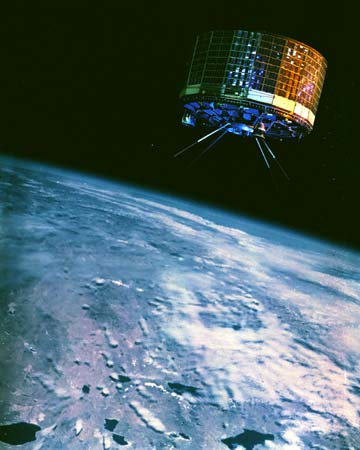
\includegraphics[scale=0.3]{TIROS_8_PAYLOAD.JPG}
        \captionof{figure}{TIROS-8 im Orbit}
    \end{center}
    Aktuell befinden sich noch drei Satelliten der US Amerikanischen Wetterbehörde Noaa in einem \glqq Low Earth Orbit\grqq(LEO). Die veraltete Technologie des Verfahrens bieten einen erleichterten Zugang im Vergleich zu heutigen Standards. Außerdem werden meist zu der Entwicklungzeit üblich niedrige Frequenzen genutzt. Das erleichtert den Empfang erheblich. Aufgrund dessen beschäftigt sich diese Arbeit mit der Vereinfachung solcher Prozesse, sowohl im Empfang als auch beim Dekodieren. Dabei sollen Prozesse in der Dekodierung beschleunigt werden, um für ein breiteres Spektrum von Meteorologen und Wissenschaftler zugänglich zu werden. Zusätzlich ist der Arbeitsablauf des Empfanges von der Antenne bis zum Dekodieren noch sehr komplex was verbessert werden soll. Es sollen weiterhin verschiedene Antennenmodell auf ihre Tauglichkeit im Bezug auf den APT Satellitenempfang getestet werden. Ich bin auf dieses Projekt gekommen, da ich mich schon seit einigen Jahren intensiv mit Hochfrequenztechnik in Satelliten beschäftige und zu Beginn oft frustriert von der vorhandenen Dokumentation im Internet war. Weiter haben mich die Antennenanforderungen förmlich erschlagen, da ich am Anfang keinerlei Erfahrungen mit Antennentechnik sowie \glqq Software definded Radios\( \grqq \) hatte. Auch fasziniert mich die Zugänglichkeit von solchen Satelliten, die keinerlei Beschränkungen wie Verschlüsselung erzwingen sondern frei empfänglich sind. Ich sehe in solchen Satelliten deshalb ein großes Potential bezogen auf Wetterstationen oder Regierungen mit wenig Mitteln für Wetterbeobachtungen, die meist nur auf Beobachtungen am Erdboden zurückgreifen müssen und so nur wage Wettervorhersagen treffen können, was zu potentiell gefährlichen Situationen führen kann. Außerdem können so Amateure eigene Daten erfassen um genauer Wetter- und Klimaveränderungen zu erfassen. Im Bezug auf die aktuellen Entwicklungen in dem Erdklima können genaue Beobachtungen getroffen werden, da die Satelliten jeden Tag zweifach über Deutschland fliegen und Daten senden.
    \newpage

\end{multicols}
\section[]{Optimierung der Software}
\begin{multicols*}{2}
    Die zu Übertragenden Daten stammen zumeist aus einem \glqq Advanced Very High Resolution Radiometer\grqq (AVHRR). Da das APT Verfahren nur einen geringen Datendurchsatz ermöglicht, werden die hochauflösenden Datenströme von dem AVHRR Instrument herunterskaliert sowie auf Graustufen umgesetzt und eignen sich deshalb für einen Transport über das APT Verfahren.  Das AVHRR der Serie 3 ist in der Lage zwischen sechs verschiedenen Spektralbändern zu differenzieren. Die Bänder reichten dabei von einer Wellenlänge von 0,58 \( \mu m\) bis 12,5 \( \mu m\) und bieten jeweils eine Auflösung von einem Pixel auf 1,1km. Kanäle 1-3A zeichnen dabei die Reflektionen der sichtbaren oder infrarotnahen Strahlen an der Erde auf. Diese Datengrundlage lässt eine Analyse der Vegetation, den Wolken, Gewässern, Schnee und Eis zu. Die verbleibenden Kanäle stellen zu einem großen Teil die Erdeigene Infrarotstrahlung dar, die von dem Meer sowie dem Land ausgestrahlt wird und genaue Temperaturwerte liefert. Die verbleibenden Instrumente sind für diese Arbeit von keiner Relevanz, da sie nicht in den entsprechenden Übertragungsverfahren ausgeliefert werden. 
    \cite{Apt-System} 
    Das Signal setzt sich aus einer Amplitudenmodulierten Niederfrequenzsignal(NF) in dem das Nutzsignal transportiert wird und dem Träger der Modulation(in diesem Fall 2.400Hz) zusammen. Das entstandene Signal wird anschließend für den Transport erneut moduliert. Diesmal wird die Frequenzmodulation aufgrund der geringeren Störungswahrscheinlichkeit gewählt. Der Träger entspricht jetzt der gewünschten Frequenz im VHF Bereich \( \approx  \)137 MHZ) und das Signal wird über eine Helix Antenne zirkular polarisiert mit wenigen Watt ausgesendet. Das Signal wird dabei aufgrund der hohen Frequenz nicht an der Ionosphäre(80-300km) reflektiert und kann somit in die Erdatmosphäre eindringen und auf der Erde empfangen werden. Es werden insgesamt 2 Linien der beiden Kanäle und zusätzliche Telemetrische Daten übertragen. So sind maximal 4160 Pixel in Grustufen pro Sekunde möglich. Anhand dieser Daten werden einfache Vorhersagen des Wetters ermöglicht. So ist die Position der Wolken genau zu bestimmen. Außerdem lässt sich die Temperatur mit einer hohen Genauigkeit extrahieren. Naturereignisse wie Vulkanmausbrücke bleiben allerdings lange unbemerkt auf den schlecht aufgelösten Bildern des APT Übertragungsverfahrens. 
    \cite{APT-How_it_works}
    Dieser Prozess wird beim Empfang der Signale revertiert und so das Eingangs erwähnte AVHRR Signal wird mit einigen Telemetriedaten sichtbar. Ich habe deshalb versucht diesen genannten Prozess selber umzusetzen und dabei eine möglichst gute Laufzeit und Nutzererfahrung meines Programms zu erreichen. Ich habe dazu Versuche in Gnu Radio durchgeführt, in denen ich anhand von Blöcken evaluiert habe. Die einzelnen Blöcke in Gnu Radio repräsentieren dabei Python- oder wahlweise C++ Code. Die Darstellung in Gnu Radio ähnelt sehr einem Fließdiagramm was die Prozesse grafisch gut und verständlich darstellen kann. So können Wissenschaftler oder Meteorologen weltweit geholfen werden, besser die Abläufe und Hintergründe der Aussendungen zu verstehen. Als zweiten Schritt soll das Flowchart in Julia einer sehr performanten Programmiersprache abgebildet werden um das Programm in der Laufzeit noch effizienter zu gestalten. Zur Hilfe nahm ich mir dabei das Flowchart von Alexandre Rouma\cite{AlexandreRouma}, sowie die Julia Bibliothek \cite[]{DSP.jl} zum Verarbeiten der Signale gleichwertig zu Gnu Radio. 

    Grundlegend bei Digitaler Signalverarbeitung ist die Abtastrate. Da Signale in Form eines Vektors digital übertragen werden, können nur eine begrenzte Anzahl an Werten innerhalb von einer Sekunde übertragen werden. Deshalb setzt sich die Einheit in der die Abtastrate angegeben wird aus einer Sekunde und den Datenpunkten innerhalb dieses Zeitfensters zusammen(\( t_s \)).
    
    Die entsprechende Abtastrate für das Flowchart habe ich aus dem Quellcode von \cite{APT-How_it_works} errechnet. Dabei bin ich auf folgende Formel gekommen.
    
    x = Eingabeabtastrate,\\ y = Ausgangsabtastrate
    \begin{equation}
        Interpolationsfaktor = GCD(x,y) / y \\
    \end{equation}
    \begin{equation}
        Dezimationsfaktor = GCD(x,y) / x 
    \end{equation}

    Die Eingangsdaten werden hierbei als WAV Datei bereitgestellt mit einer Abtastrate von 37500(\( t_s \)). Das Shannon-Abtasttheorem beschreibt dabei, dass ein Sinusförmiges Signal bei doppelter Abtastrate von der Eingangsfrequenz komplett repräsentiert werden kann. Diese Eigenschaft können wir uns auch zunutze machen und die Abtastrate auf theoretisch 11025\( t_s \) beschränken. So reduziert man Beispielsweise den Datensatz um das dreifache ohne theoretisch merkbare Qualitätsverluste. Die Abtastrate von 11025\( t_s \) durch das doppelte von der maximalen Nutzfrequenz, die sich aus dem Träger von 2400Hz und dem Signal(3112.5Hz) zusammensetzt. Das bedeutet eine deutlich schnellere Laufzeit da unnötige Iterationen eingespart werden können. Ein ähnliches Verfahren wird auch bei analogen Empfängern verwendet, um leichter das Signal verändern zu können, weil Oszillatoren mit einer hohen Frequenz die Tendenz besitzen stärker in der Frequenz zu schwanken. 
    Abb. 2 ist zwar etwas Zeitversetzt zeigt aber anhand der Stärke der Farbe, dass bei gleichbleibender Qualität weniger Abtastpunkte benötigt werden. Um noch mehr Abtastpunkte einzusparen, wird das Signal gegen eine Signalquelle gemischt um so eine maximale Arbeitsfrequenz(NF) von 3112.5Hz zu erhalten. Da das Signal auf beiden Seitenbändern aufmoduliert ist, können wir uns auf das obere beschränken und so eine Abtastrate von 6225Hz nutzen. Wir erhalten nachdem wir die Formel angewand haben einen Interpolationsfaktor von 83 und einen Dezimationsfaktor von 147. Dabei ist zu beachten das wir keine Abtastpunkte löschen können, da wir sonst die Frequenz verändern und so alle nachfolgenden Signalverarbeitungsschritte angepasst werden müssten.

    So konnte zum ursprünglichen Algorithmus die Abtastrate um den Faktor 3,5 reduziert werden, was die Anzahl der Iterationen im darunterliegenden Code um den gleichen Faktor mindert. Die Dateigröße bei einer Aufnahme mit 3750 \( t_s \) sollte auch die Dateigröße der Eingangsdatei maßgeblich reduzieren. Bei genauerer Betrachtung der Resultate ist ein leichter Qualitätsverlust erkennbar. Dieser Resultiert womöglich aus der Nutzung der theoretischen Mindestabtastrate. Bei den Berechnungen nicht berücksichtigt wurden mögliche Ungenauigkeiten wie der Dopplereffekt, der die Aufnahme verzerrt, oder Effekte die bei der Digitalen Signalverarbeitung entstanden sind. Außerdem werden Artefakte von dem Sinusförmigen Signal mit einer Frequenz von -1.4MHz in das Nutzsignal gemischt. Um Trotzdem eine unveränderte Bildqualität zu erreichen, hat sich der dreifache Wert des theoretischen Minimums als beste Balance zwischen Qualität und Leistung herausgestellt.
    Ich habe anschließend versucht das Flowchart auch in Julia zu replizieren. Dazu habe ich die Daten und die Abtastrate aus der WAV Datei importiert und so einen Array aus Floats mit einer Größe von jeweils 64Bit bekommen. Der Wertebereich reicht dabei von 1.0 bis -1.0.
   
    \begin{math}
        \mathbf{W} =[-1.0, 1.0]
    \end{math}

    Jeder Zahl in dem Vektor belegt im Heap(meist im Arbeitsspeicher) 64Bits und ist um das doppelte genauer wie die vergleichbare Implementation in Gnu radio die eine Auflösung von 32bit liefert. 

    \begin{math}
        \begin{bmatrix}
            -0.35938596758934294;\\
            -0.7111117893002106;\\
            0.25470748008667254;\\
            0.5893124179815058;\\
        \end{bmatrix}
    \end{math}

    Bei dem Quellcode habe ich mich aufgrund fehlender Dokumentation von dem DSP(digital signal processing) Paket stark an der Arbeit von \cite[]{APTDecoder.jl}orientiert. Um auch in dieser Implementation an das Niederfrequenzsignal aus der Amplitudenmodulation zu kommen, verwende ich die Hilbert Transformation. Diese setzt das Signal in ein komplexes Signal um, welches aus einer Amplitude und einem Phasenwinkel besteht. Da die Hochfrequenz nur in den Phasenwinkel umgesetzt wird, können wir den Amplitudenwert als demoduliertes Niederfrequenzsignal weiterverarbeiten. Die Filter in Julia DSP bestehen dabei aus der Filterart wie einem Bandpass in diesem Fall und einem Filtertyp einem Butterworth Filter. Der Filtertyp bestimmt dabei die Eigenschaften des Filters, so definiert er die Passbandfrequenzen und die Steigung an den Flanken des gefilterten Bereiches. Da wir das Eingangssignal filtern um keine unnötigen Störungen in der Hilbert Transformation zu erzeugen beschränken wir uns mithilfe des Bandpasses auf den Bereich von 400Hz bis 4400Hz. Nachdem das Signal demoduliert wurde, kann ein Neuabtastung mit einer geringeren Abtastrate dabei helfen den Synchronisationsvorgang zu erleichtern. Ich behelfe mich dabei der Funktion 1. und 2. Der verwendete Code um die Arrays in eine richtige Anordnung zu bringen habe ich komplett von \cite[]{APTDecoder.jl} übernommen. So entstehen mehrdimensionale Vektoren die in Grasstufen umgesetzt und gespeichert werden können. Siehe Abb.5.
    Da der Julia Compiler sehr viele Überprüfungen zur Übersetzungszeit ausführt, dauert der Testprozess sehr lange was den Einstieg erschwert. Außerdem werden die Abhängigkeiten schon vorab kompiliert war zusätzlich die Übersetzungszeit verlängert. Die Benutzung wird aber erleichtert, da keine Speicherlecks mehr möglich sind und die Laufzeit durch eine vorab Kompilierung verbessert wird. Aber die Bildergebnisse wurden deutlich verbessert außerdem konnte eine deutliche Reduktion der Laufzeit festgestellt werden. So erreicht Julia C ähnliche Leistungen was sich deutlich in der Auslastung von Systemressourcen zeigt. 
\end{multicols*}
    
\begin{center}
    \centering
    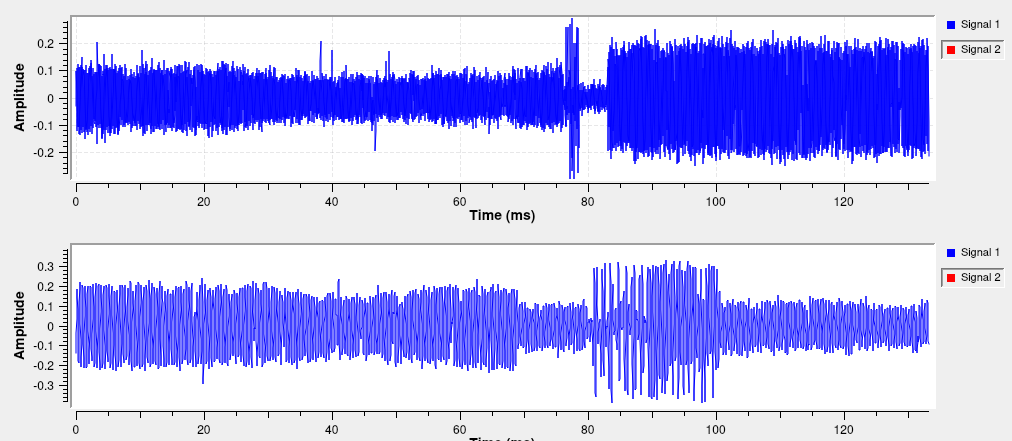
\includegraphics[scale=0.3]{20220103164144.png}
    \captionof{figure}{Abtastraten im Vergleich 
    oben:37500 \( t_s \)\\ unten: 11025\( t_s \)}
\end{center} 
\begin{center}
    \centering
    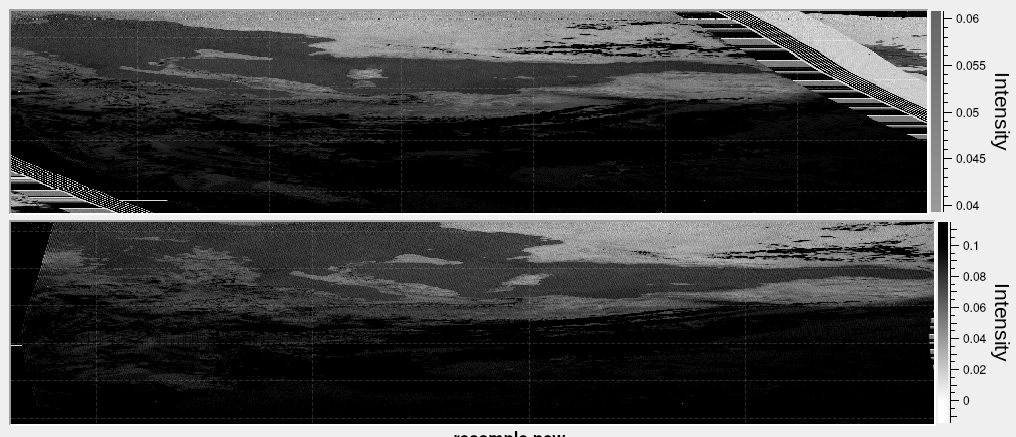
\includegraphics[scale=0.3]{20220110214426.png}
    \captionof{figure}{Endergebnis im Vergleich 
    oben:3112 \( t_s \)\\ unten: 11025\( t_s \)}
\end{center}

\begin{center}
    \centering
    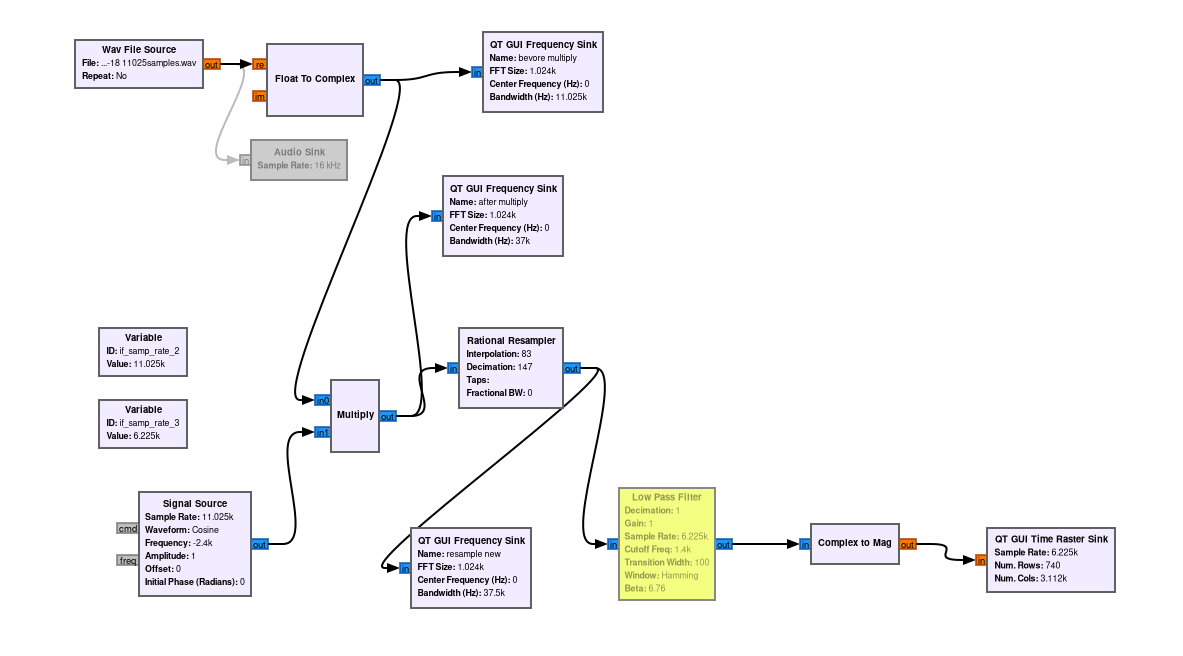
\includegraphics[scale=0.3]{20220115213521.png}
    \captionof{figure}{Der Flowchart in Gnuradio.}
\end{center}

\begin{center}
    \centering
    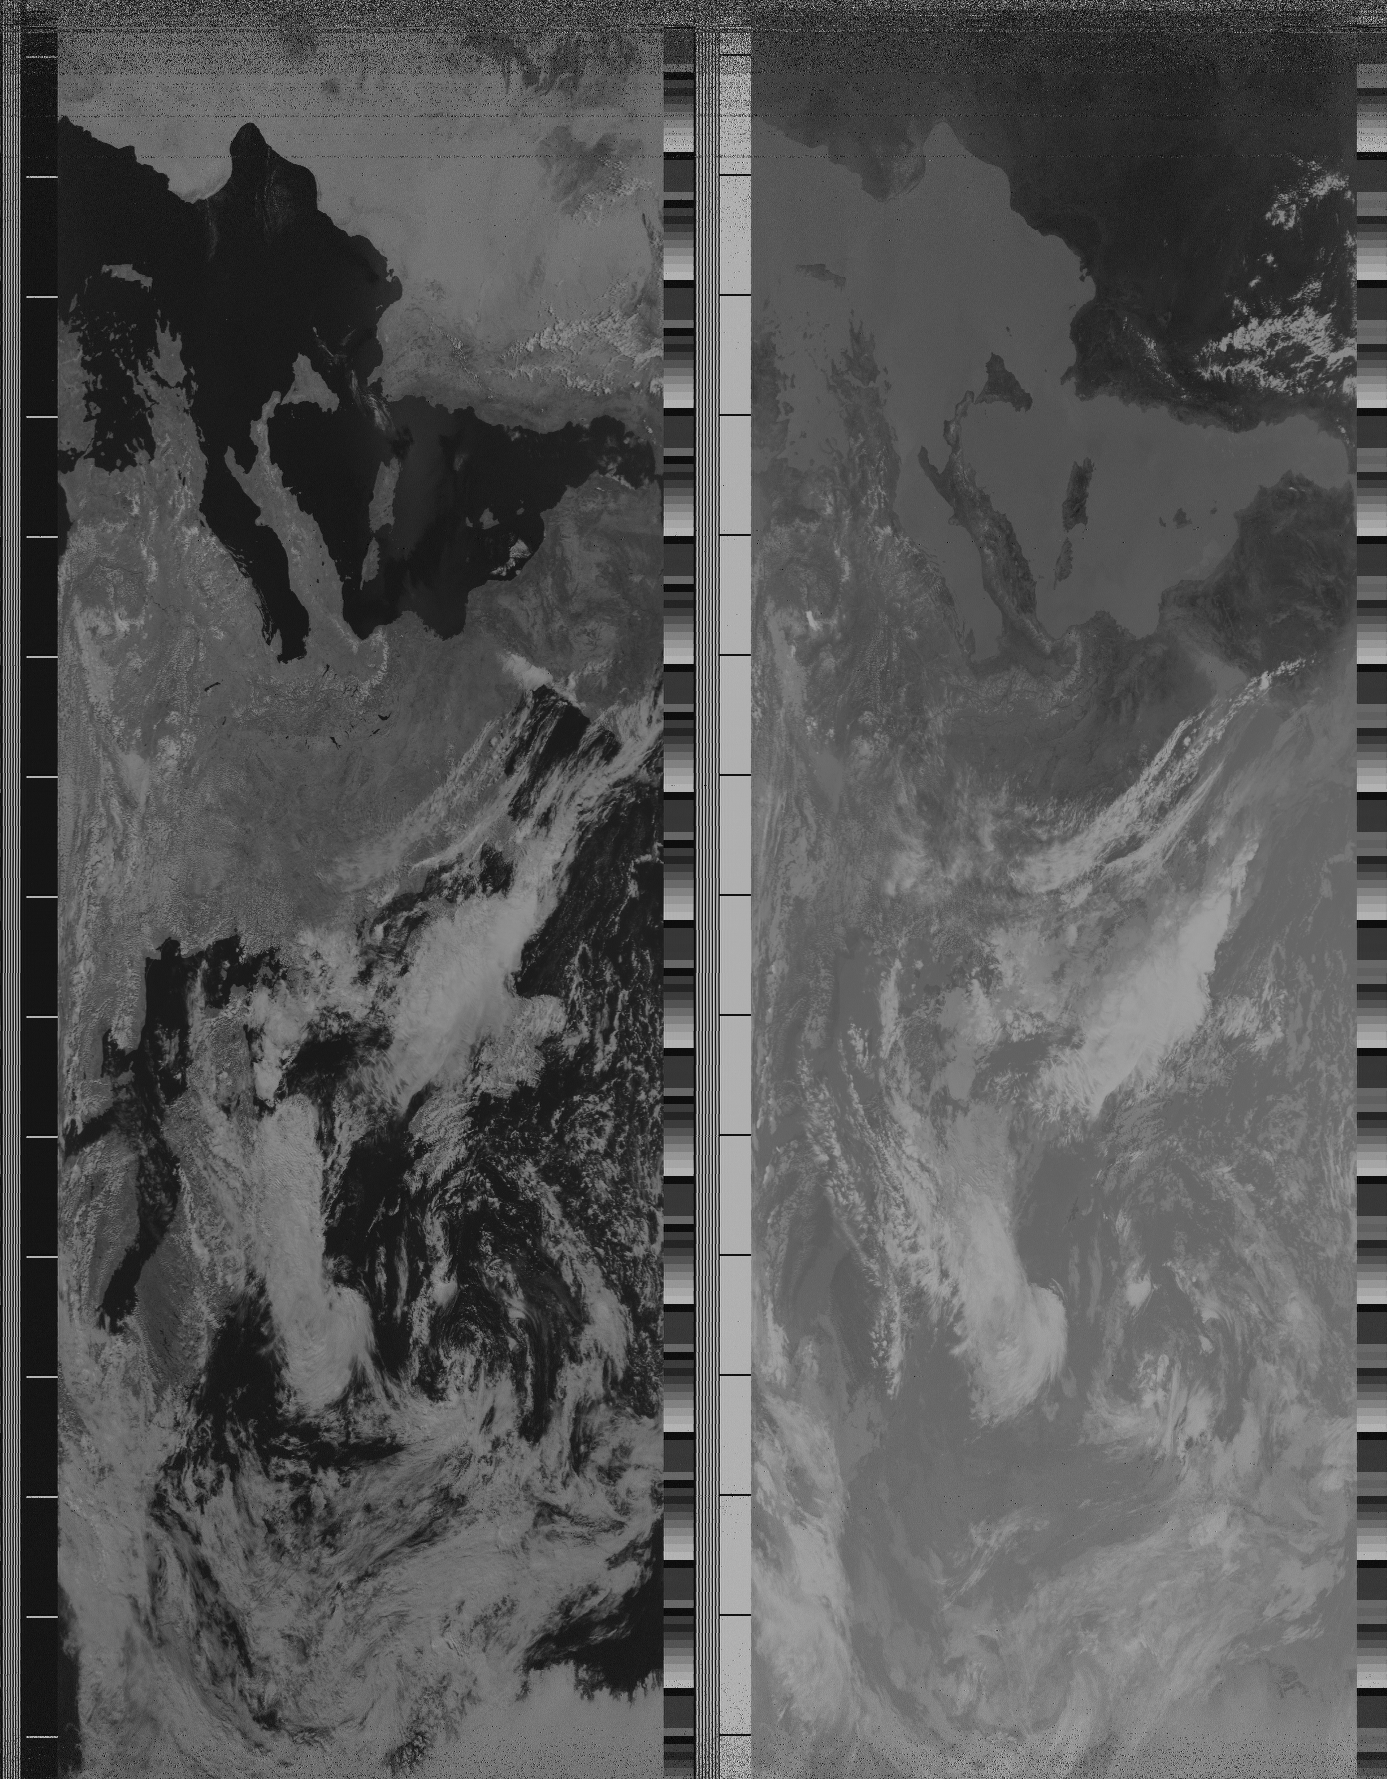
\includegraphics[scale=0.18]{test.png}
    \captionof{figure}{Ergebnis des Julia Programes.}
\end{center}

\section[]{Optimierung der Antennen}

\begin{multicols*}{2}
    Einer der wichtigsten Faktoren ist neben der Empfindlichkeit des Empfängers die Charakteristiken der verwendeten Antenne. In dem folgenden Abschnitt habe ich verschiedene Antennen verglichen und sie auf Tauglichkeit sowie ihre Anwendbarkeit geprüft. Die erste Bauweise die ich analysiert habe ist die sogenannte V-Dipol Antenne die eine starke Ähnlichkeit zu einer gewöhnlichen Dipol Antenne besitzt. Ich habe mich aufgrund der besseren Reproduzierbarkeit dieser Arbeit dazu entschieden die Antenne selber zu bauen. Die nötigen Daten lassen sich mithilfe der Formel 3 und 4 berechnen. X muss dabei immer einem vielfachen von 2 entsprechen um die Verhältnisse zu wahren. 299792458m/s entspricht der Ausbreitungsgeschwindigkeit von Elektromagnetischen Wellen also annähernd der Lichtgeschwindigkeit. Das Ergebnis der Gleichung ist in Nanometern zu verstehen, so erhalten wir bei einer Mittelfrequenz von 137MHz unserer Antenne, eine Länge von insgesamt 2188266nm. Da wir den größtmöglichen Gewinn bei der Antenne erreichen wollen, nutzen wir den Divisor 2 bei Funktion 4 und erhalten so eine Länge von insgesamt 1,094133m. Jedes Element entspricht also 5,
    47066m.
    \newpage
    

    \begin{equation}
        \lambda = \frac{299792458 m/s}{f}  
    \end{equation}


    \begin{equation}
        \frac{\lambda}{x}  
    \end{equation}

    Um die Elemente mit dem Radio in unserem Fall einem Software Defined Radio(SDR) zu verbinden, nutzen wir einfaches RG58 Koaxialkabel welches einen relativ hohen Dämpfungsfaktor bei hohen Frequenzen besitzt. Deshalb versuchen wir den Abschnitt zwischen dem Radio und der Antenne möglichst gering zu halten. So kann der Verlust reduziert werden und die Einstrahlung vermindert werden. Beide Elemente aus Kupferdraht können über einen handelsüblichen Kabelverbinder mit dem Koaxialkabel verbunden werden. Hierzu ist kein Löten nötig, aber es ist der Stabilität sehr zuträglich. Weiterhin muss eine gewisse Richtwirkung der Antenne bestehen um das Signal zu Rauschen Verhältnis zu verbessern. Die genauen Angaben zu dem Verhältnis der beiden Elemente zueinander, habe ich aus \cite[]{Diy137MHz} bezogen. 

    Nach einigen Tests ist die Richtwirkung beim Empfang stark aufgefallen, so muss der Satellit in seinem Orbit verfolgt werden um die besten Ergebnisse zu erhalten. Außerdem konnte man die falsche Polarisation der Antenne bemerken, die einen geringen Verlust an Signal zu Rausch Verhältnis zur Folge hat. Das Signal wird zirkular polarisierend von den Satelliten ausgesendet, die Antenne aber ist nur linear polarisiert durch ihre flache Bauweise. Eine helixförmige Antenne würde die richtige Polarisation aufweisen, ist aber auch entsprechend kompliziert zu bauen und wurde aus diesen Gründen nicht in diesem Projekt einbezogen. 

    Eine weiter Möglichkeit die klassische Dipol Antenne zu variieren, besteht darin, diese zu doppeln und in Form einer Kreuzdipolantenne zu bauen. Die getestete Kreuzdipolantenne hat sich außerordentlich schlecht für Satellitenempfang geeignet, da sie nur den Bereich über zentral Europa Abdecken konnte. Ein Grund ist womöglich die schlechte Richtwirkung, diese Resultiert aus den immer gleichbleibenden Winkeln zwischen den Elementen der Antenne. 

\end{multicols*}


\begin{center}
    \centering
    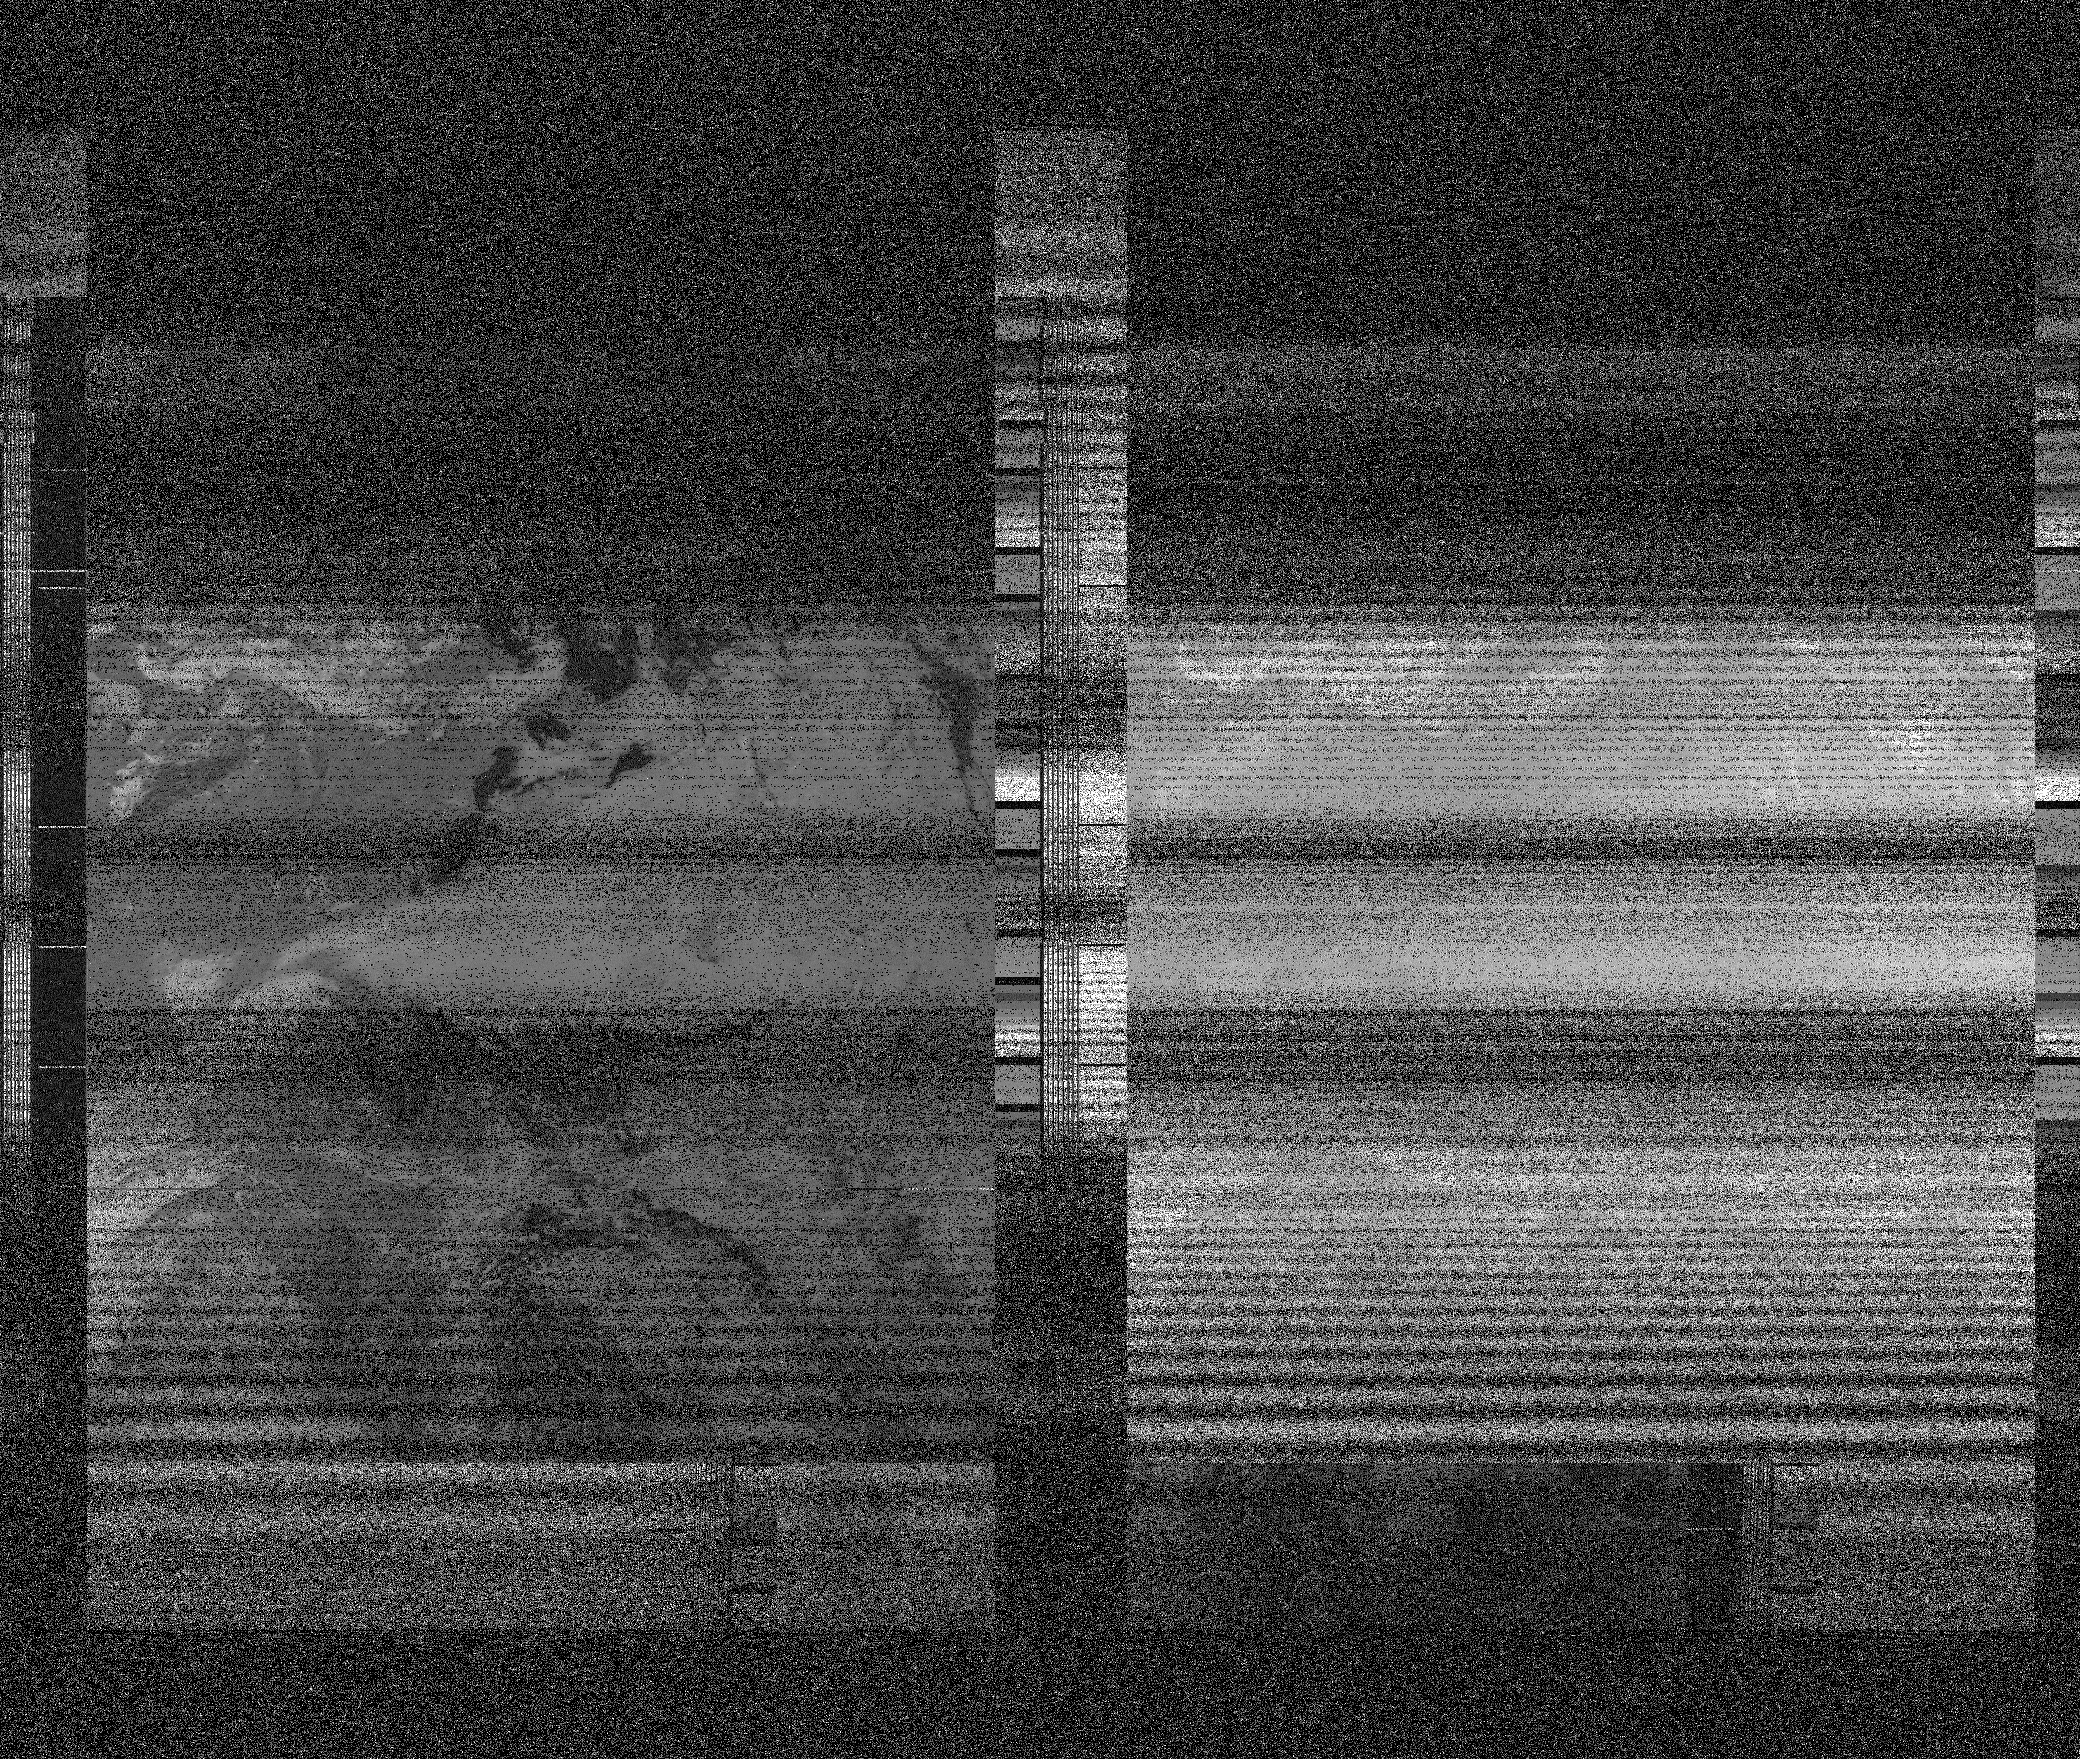
\includegraphics[scale=0.14]{Kreuzdipol.png}
    \captionof{figure}{Ein Überflug empfangen mit der Kreuzdipolantenne.}
\end{center}

\begin{center}
    \centering
    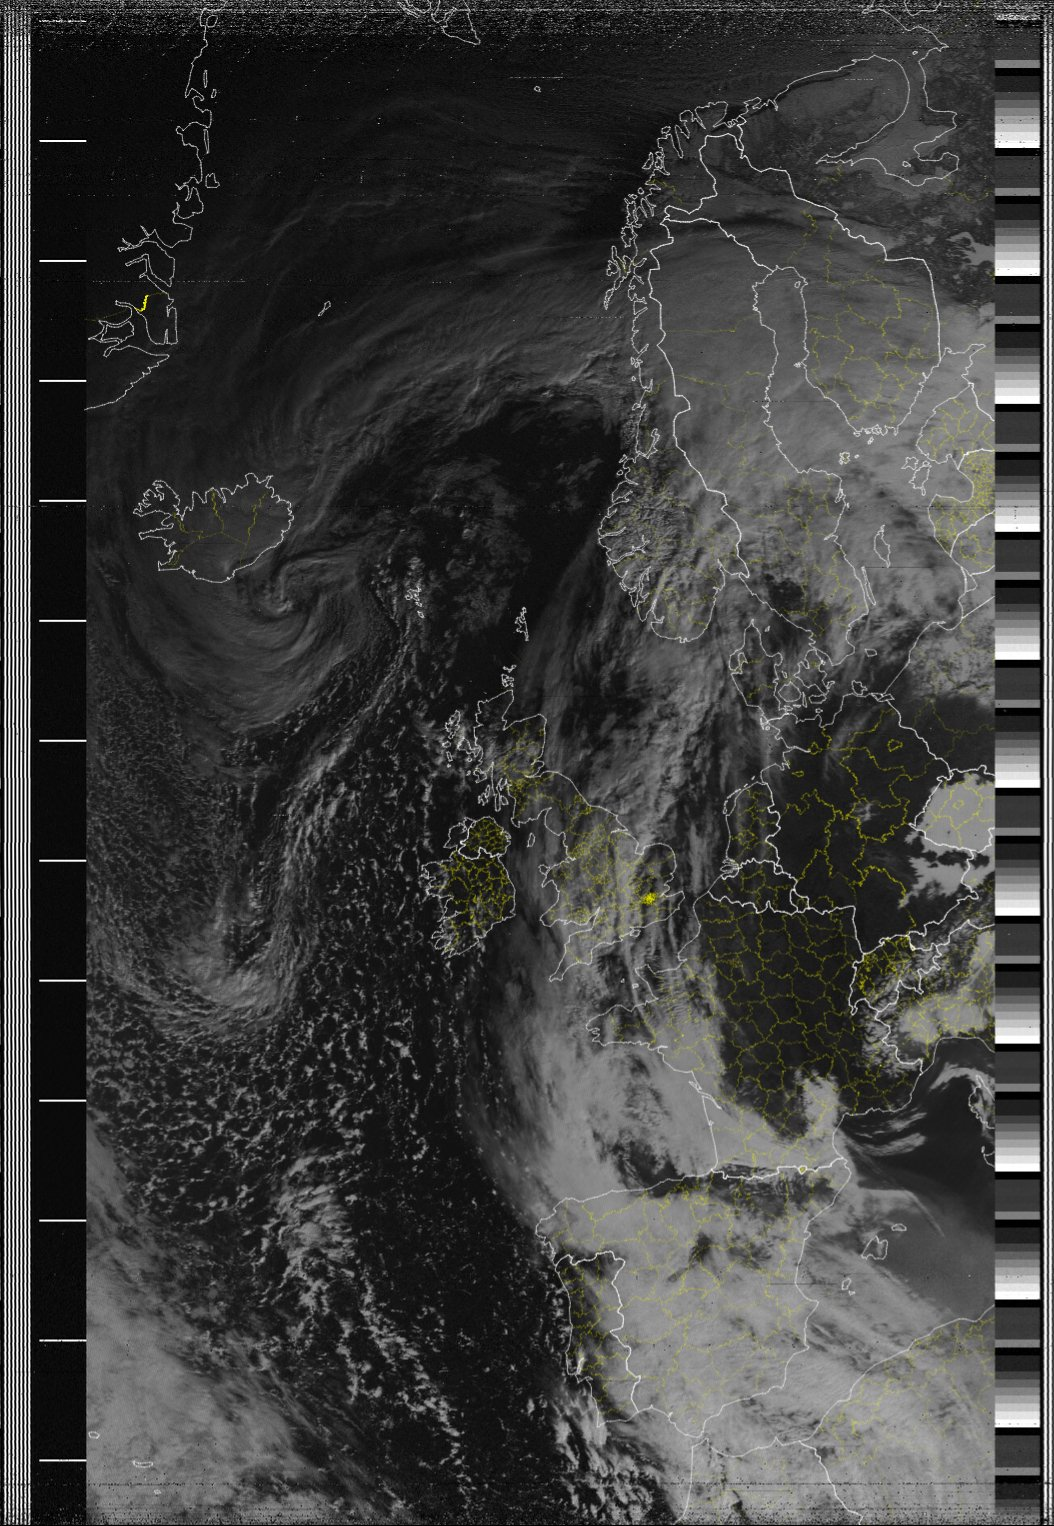
\includegraphics[scale=0.14]{nooa.jpg}
    \captionof{figure}{Ein Überflug empfangen mit der V-Dipolantenne.}
\end{center}


\part{Zukunft}
\section[]{High-resolution picture transmission(HRPT)}

Hrpt beschreibt den Nachfolger des APT Verfahrens. Es setzt im Vergleich zu diesem auf eine digitale Übertragung der Daten. Die Signale werden im L-Band auf Frequenzen um 1,7GHz ausgesendet. Die Übertragungen beschränken sich aber auf einfache Bilddaten in verschiedenen Wellenlängen des visuellen und infraroten Spektrums. Die Daten sind zu einem großen Teil die selben wie aus dem APT Verfahren aber mit einer deutlich erhöhten Qualität. Deshalb setzten neben Noaa auch Europäische Wetterorganisationen auch heute noch auf dieses Verfahren. Da die Antennen sehr klein werden wird eine Satellitenschüssel erforderlich um die Verluste der kleinen Antenne zu kompensieren. Hierzu eignet sich auch eine Helix Antenne die aufgrund der kleinen Größe einfacher zu bauen ist als für 137Mhz. Leider bewegt sich der Trend immer weiter weg von einfach zu empfangenden Signalen, die mit wenig Aufwand empfangen werden können. Das hat zum einen den Grund des deutlich erhöhten Datendurchsatzes in höheren Frequenzen. Zum anderen den technischen Fortschritt in Bezug auf die Dekodierungsverfahren sowie die Modulationsverfahren.  


\part*{Danksagung}

Ich bedanke mich bei meinem Onkel der mich beim Bau der Antennen unterstützt hat und mir die Kreuzdipolantenne zur Verfügung gestellt hat.